\label{sec:resultsMulti}

\subsection{Overview}

Figure~\ref{fig:simresultsmulti_nominal} shows the complete MultiFolded results, with all 24 observables and their total systematic uncertainty (see Sec.~\ref{sec:multifolduncerts} for details).  Note that the results are unbinned and simultaneous, but for illustration, we use the binning introduced in Sec.~\ref{sec:pres} and plot one observable at a time.  Sherpa is used as data and Pythia is used as the simulation.  Overall, the closure (comparison of filled and unfilled histograms) is excellent across the entire phase space.

\begin{figure}[h!]
\centering
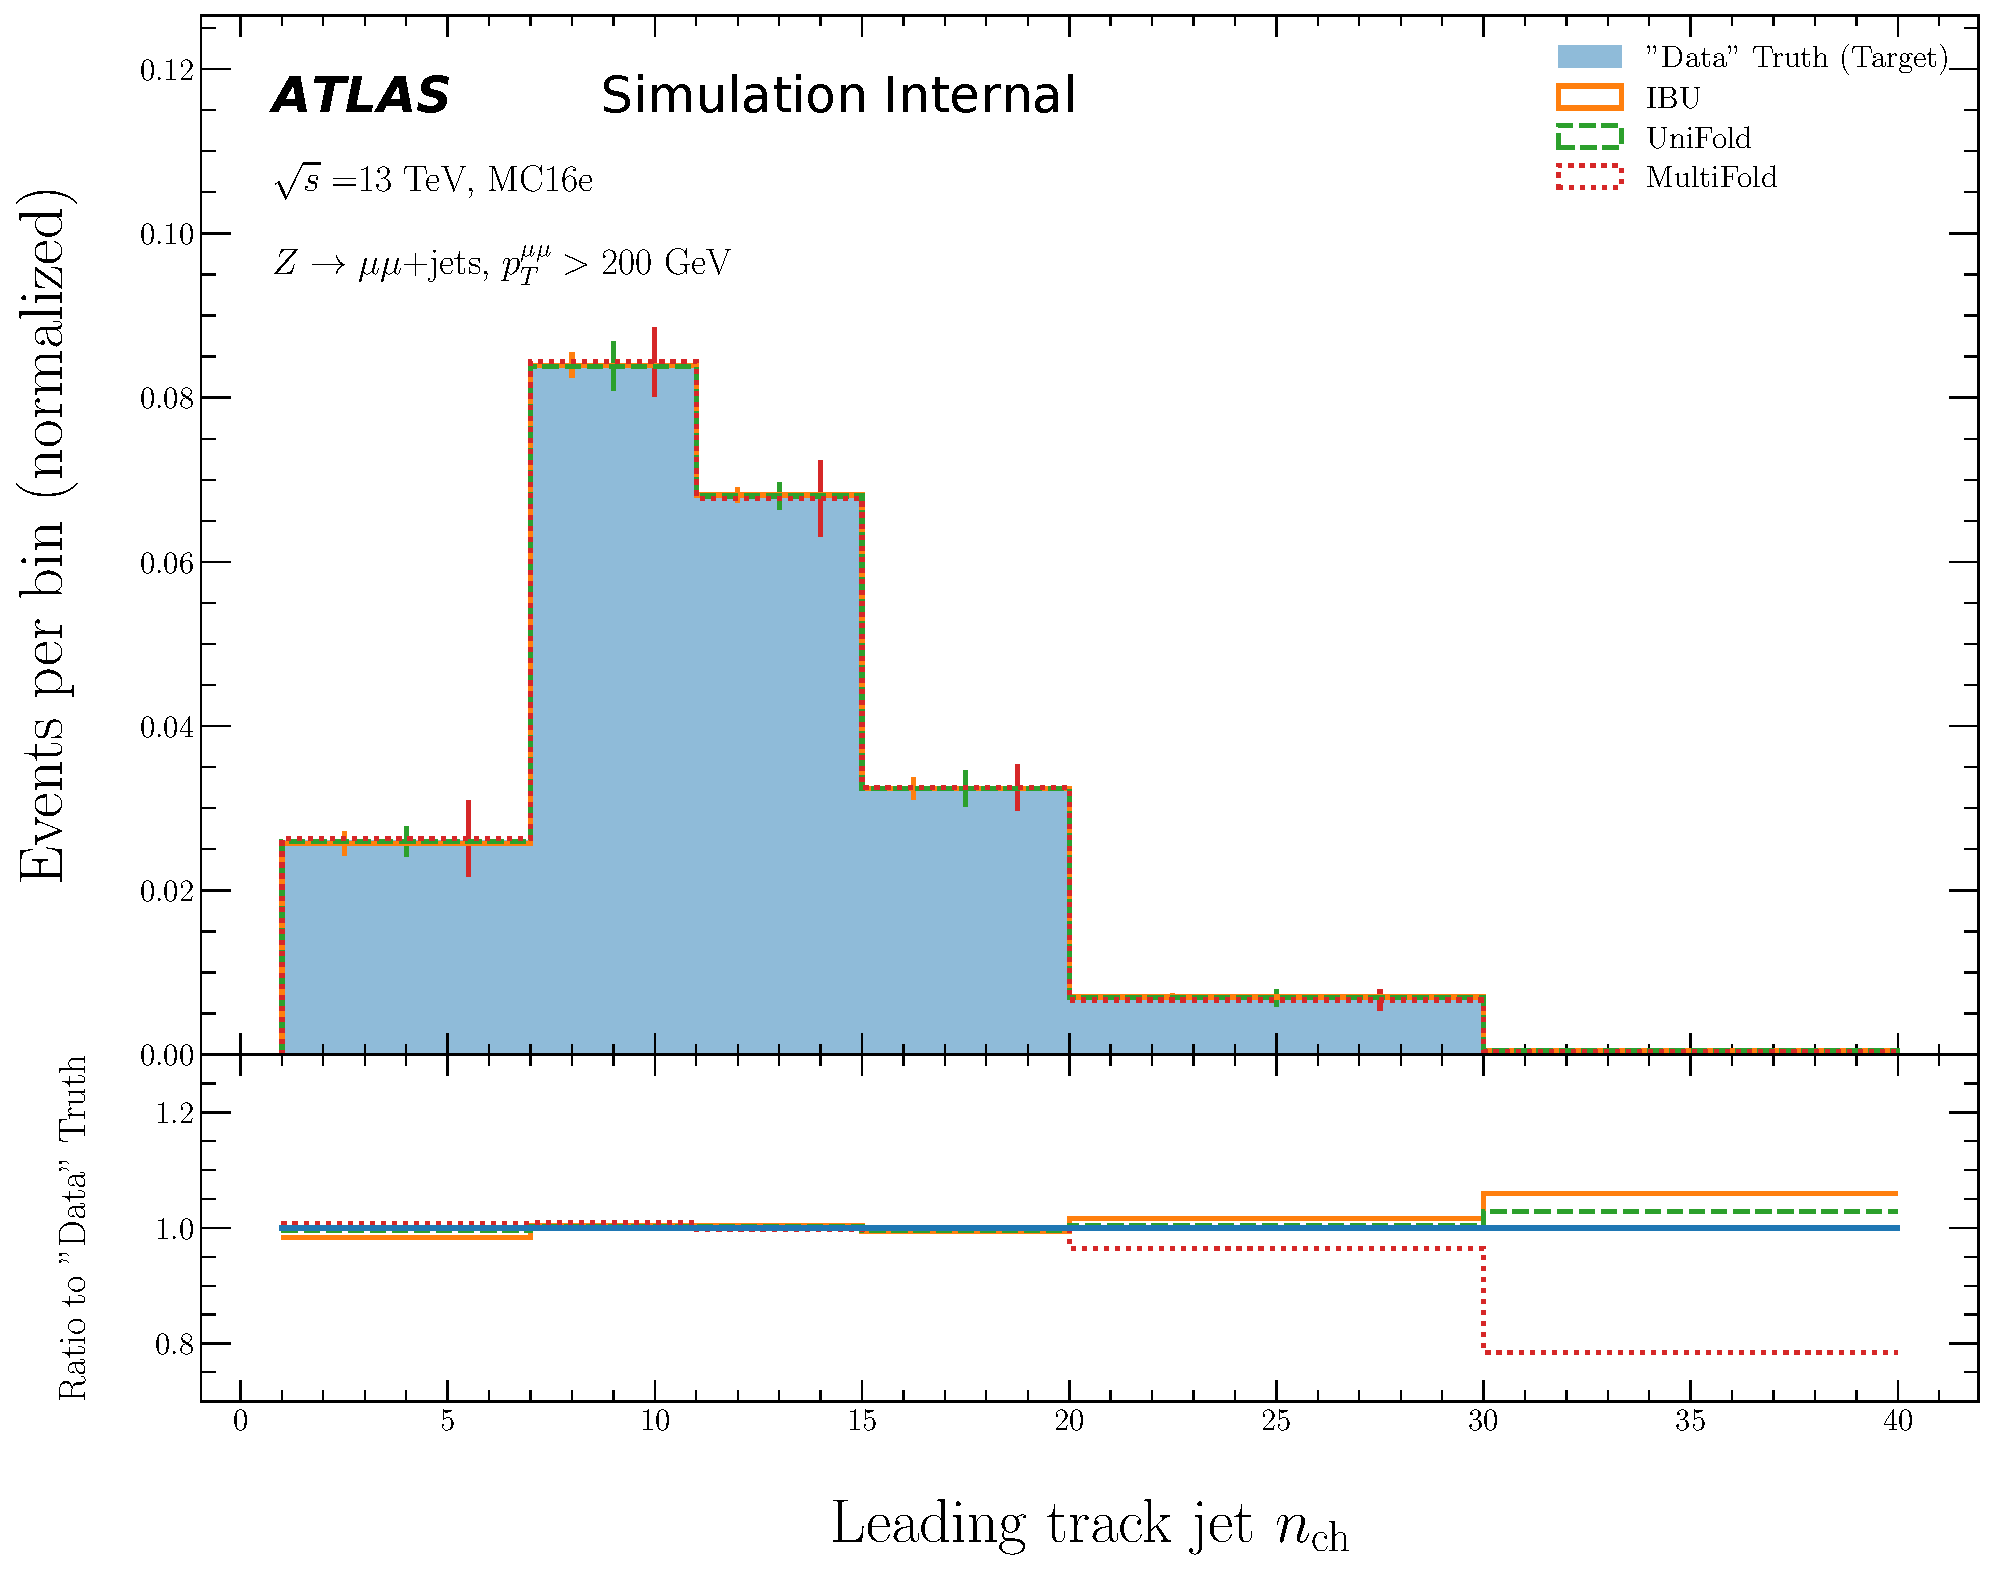
\includegraphics[width=0.25\textwidth,page=1]{figures/SimResults/TotalErrors.pdf}\includegraphics[width=0.25\textwidth,page=2]{figures/SimResults/TotalErrors.pdf}\includegraphics[width=0.25\textwidth,page=3]{figures/SimResults/TotalErrors.pdf}\includegraphics[width=0.25\textwidth,page=4]{figures/SimResults/TotalErrors.pdf}\\
\includegraphics[width=0.25\textwidth,page=5]{figures/SimResults/TotalErrors.pdf}\includegraphics[width=0.25\textwidth,page=6]{figures/SimResults/TotalErrors.pdf}\includegraphics[width=0.25\textwidth,page=7]{figures/SimResults/TotalErrors.pdf}\includegraphics[width=0.25\textwidth,page=8]{figures/SimResults/TotalErrors.pdf}\\
\includegraphics[width=0.25\textwidth,page=9]{figures/SimResults/TotalErrors.pdf}\includegraphics[width=0.25\textwidth,page=10]{figures/SimResults/TotalErrors.pdf}\includegraphics[width=0.25\textwidth,page=11]{figures/SimResults/TotalErrors.pdf}\includegraphics[width=0.25\textwidth,page=12]{figures/SimResults/TotalErrors.pdf}\\
\includegraphics[width=0.25\textwidth,page=13]{figures/SimResults/TotalErrors.pdf}\includegraphics[width=0.25\textwidth,page=14]{figures/SimResults/TotalErrors.pdf}\includegraphics[width=0.25\textwidth,page=15]{figures/SimResults/TotalErrors.pdf}\includegraphics[width=0.25\textwidth,page=16]{figures/SimResults/TotalErrors.pdf}\\
\includegraphics[width=0.25\textwidth,page=17]{figures/SimResults/TotalErrors.pdf}\includegraphics[width=0.25\textwidth,page=18]{figures/SimResults/TotalErrors.pdf}\includegraphics[width=0.25\textwidth,page=19]{figures/SimResults/TotalErrors.pdf}\includegraphics[width=0.25\textwidth,page=20]{figures/SimResults/TotalErrors.pdf}\\
\includegraphics[width=0.25\textwidth,page=21]{figures/SimResults/TotalErrors.pdf}\includegraphics[width=0.25\textwidth,page=22]{figures/SimResults/TotalErrors.pdf}\includegraphics[width=0.25\textwidth,page=23]{figures/SimResults/TotalErrors.pdf}\includegraphics[width=0.25\textwidth,page=24]{figures/SimResults/TotalErrors.pdf}
\caption{The nominal MultiFolded results where Sherpa is used as data and Pythia is used as the simulation. The error bars represent the total uncertainty, which each component added in quadrature.}
\label{fig:simresultsmulti_nominal}
\end{figure}

%%%

\begin{comment}
\begin{figure}[h!]
\centering
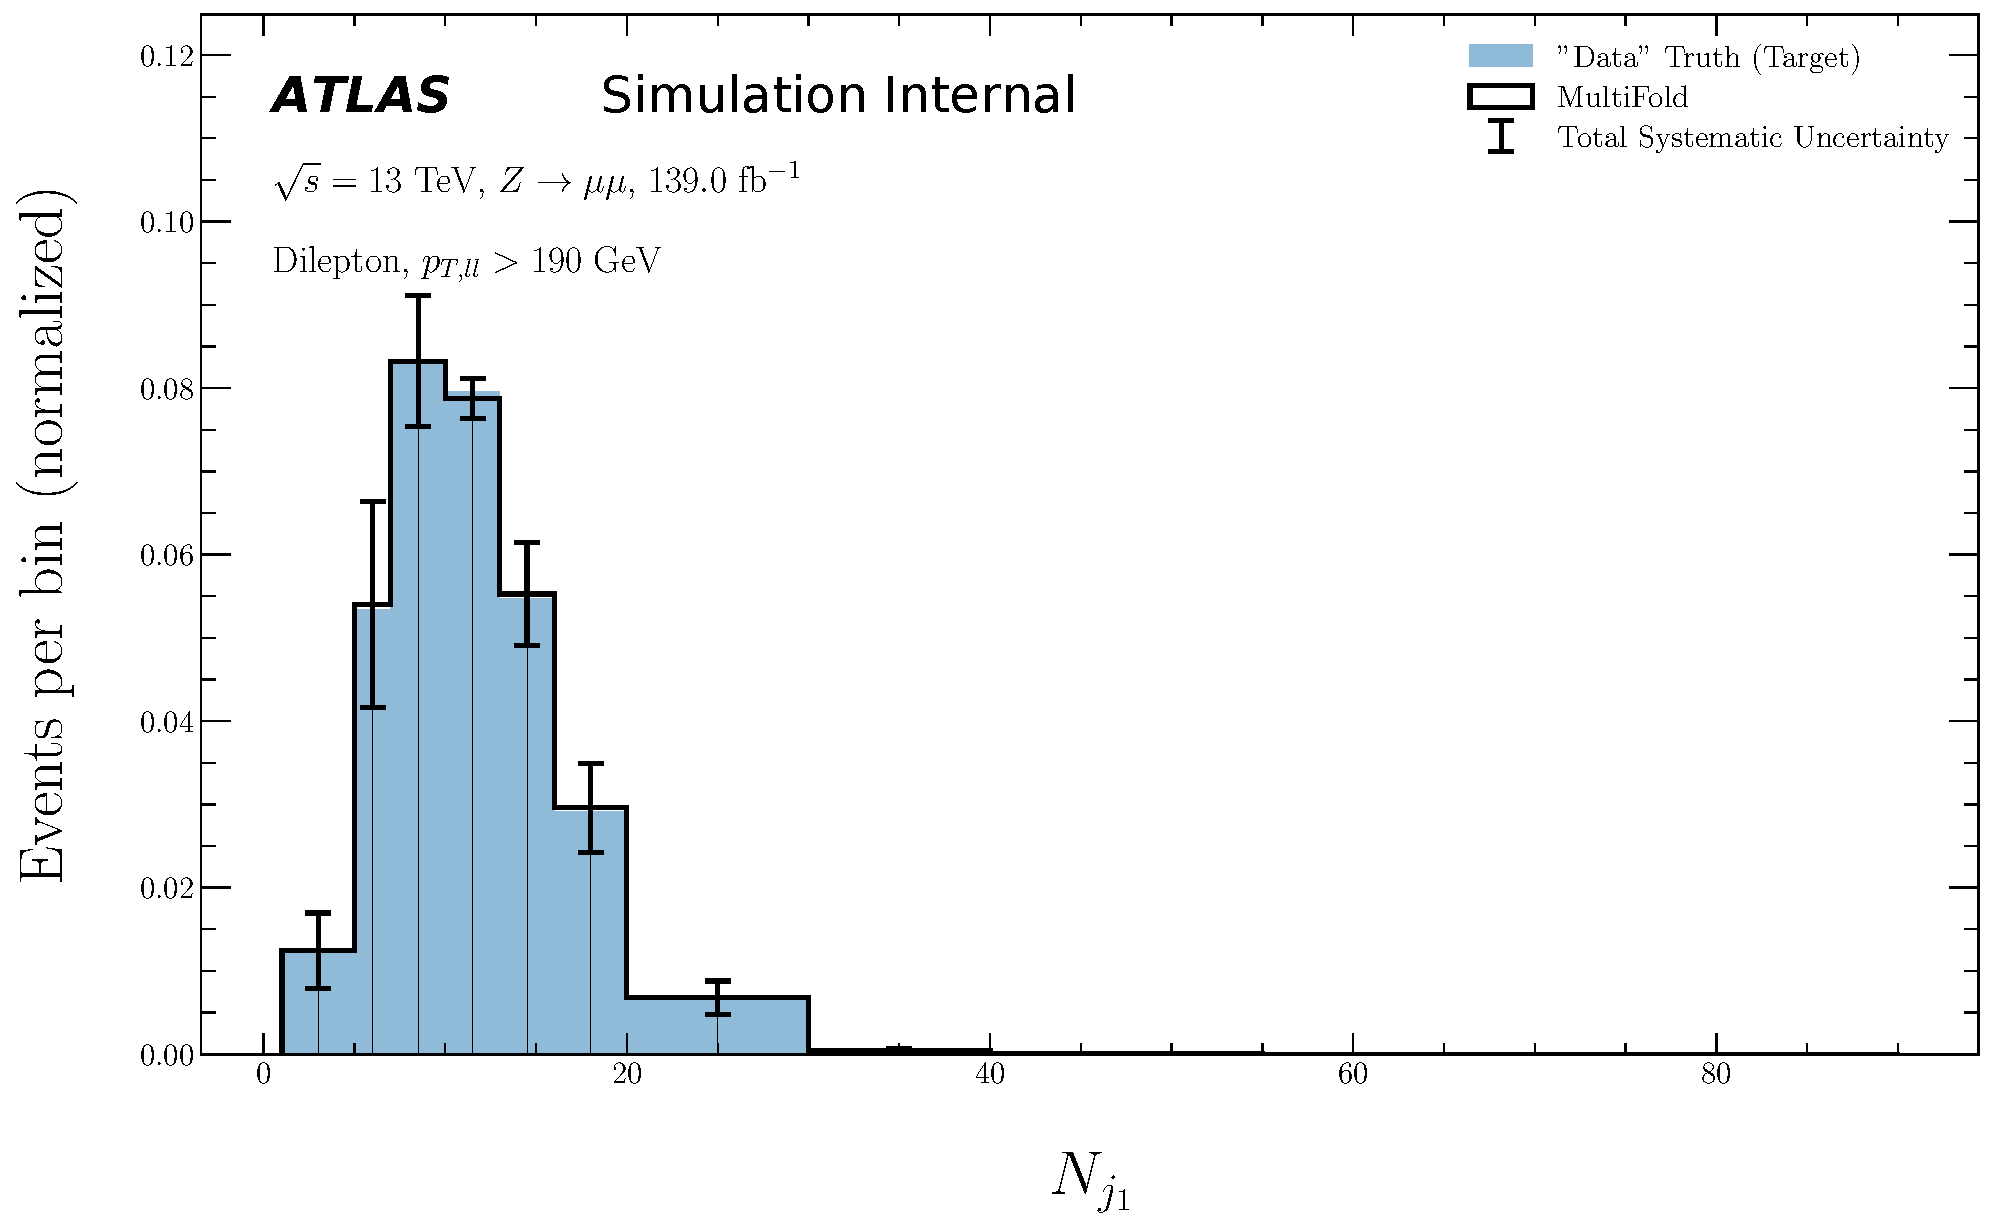
\includegraphics[width=0.25\textwidth,page=1]{figures/SimResults/MultiFoldTotalErrors.pdf}\includegraphics[width=0.25\textwidth,page=2]{figures/SimResults/MultiFoldTotalErrors.pdf}\includegraphics[width=0.25\textwidth,page=3]{figures/SimResults/MultiFoldTotalErrors.pdf}\includegraphics[width=0.25\textwidth,page=4]{figures/SimResults/MultiFoldTotalErrors.pdf}\\
\includegraphics[width=0.25\textwidth,page=5]{figures/SimResults/MultiFoldTotalErrors.pdf}\includegraphics[width=0.25\textwidth,page=6]{figures/SimResults/MultiFoldTotalErrors.pdf}\includegraphics[width=0.25\textwidth,page=7]{figures/SimResults/MultiFoldTotalErrors.pdf}\includegraphics[width=0.25\textwidth,page=8]{figures/SimResults/MultiFoldTotalErrors.pdf}\\
\includegraphics[width=0.25\textwidth,page=9]{figures/SimResults/MultiFoldTotalErrors.pdf}\includegraphics[width=0.25\textwidth,page=10]{figures/SimResults/MultiFoldTotalErrors.pdf}\includegraphics[width=0.25\textwidth,page=11]{figures/SimResults/MultiFoldTotalErrors.pdf}\includegraphics[width=0.25\textwidth,page=12]{figures/SimResults/MultiFoldTotalErrors.pdf}\\
\includegraphics[width=0.25\textwidth,page=13]{figures/SimResults/MultiFoldTotalErrors.pdf}\includegraphics[width=0.25\textwidth,page=14]{figures/SimResults/MultiFoldTotalErrors.pdf}\includegraphics[width=0.25\textwidth,page=15]{figures/SimResults/MultiFoldTotalErrors.pdf}\includegraphics[width=0.25\textwidth,page=16]{figures/SimResults/MultiFoldTotalErrors.pdf}\\
\includegraphics[width=0.25\textwidth,page=17]{figures/SimResults/MultiFoldTotalErrors.pdf}\includegraphics[width=0.25\textwidth,page=18]{figures/SimResults/MultiFoldTotalErrors.pdf}\includegraphics[width=0.25\textwidth,page=19]{figures/SimResults/MultiFoldTotalErrors.pdf}\includegraphics[width=0.25\textwidth,page=20]{figures/SimResults/MultiFoldTotalErrors.pdf}\\
\includegraphics[width=0.25\textwidth,page=21]{figures/SimResults/MultiFoldTotalErrors.pdf}\includegraphics[width=0.25\textwidth,page=22]{figures/SimResults/MultiFoldTotalErrors.pdf}\includegraphics[width=0.25\textwidth,page=23]{figures/SimResults/MultiFoldTotalErrors.pdf}\includegraphics[width=0.25\textwidth,page=24]{figures/SimResults/MultiFoldTotalErrors.pdf}
\caption{The nominal MultiFolded results where Sherpa is used as data and Pythia is used as the simulation. The error bars represent the total uncertainty, which each component added in quadrature.}
\label{fig:simresultsmulti_nominal}
\end{figure}
\end{comment}

\subsection{Systematic Uncertainites}
\label{sec:multifolduncerts}

This section contains a per-observable systematic uncertainty breakdown.  Note that like the central values from the previous section, the uncertainties are unbinned.  The binning is for illustration only and matches the one used in the previous section.  The experimental systematic uncertainties are illustrated in Figs.~\ref{fig:simresultsmulti_trackjetuncertsl} and~\ref{fig:simresultsmulti_muonuncerts}, for the inclusive tracking and muon reconstruction, respectively.  For the inclusive tracking uncertainties, the most important are the inclusive tracking efficiency (\texttt{sys\_TrackFilter}) and the sagitta bias (\texttt{sys\_pTScale}).  For some of the uncertainties, we do not expect a large dependence on $\phi$ and therefore the fluctuations seen for the jet and lepton $\phi$ observables are an indication of the small $\mathcal{O}(1\%)$ variations introduced by the neural network training.  This may be improved with further regularization.

\begin{figure}[h!]
\centering
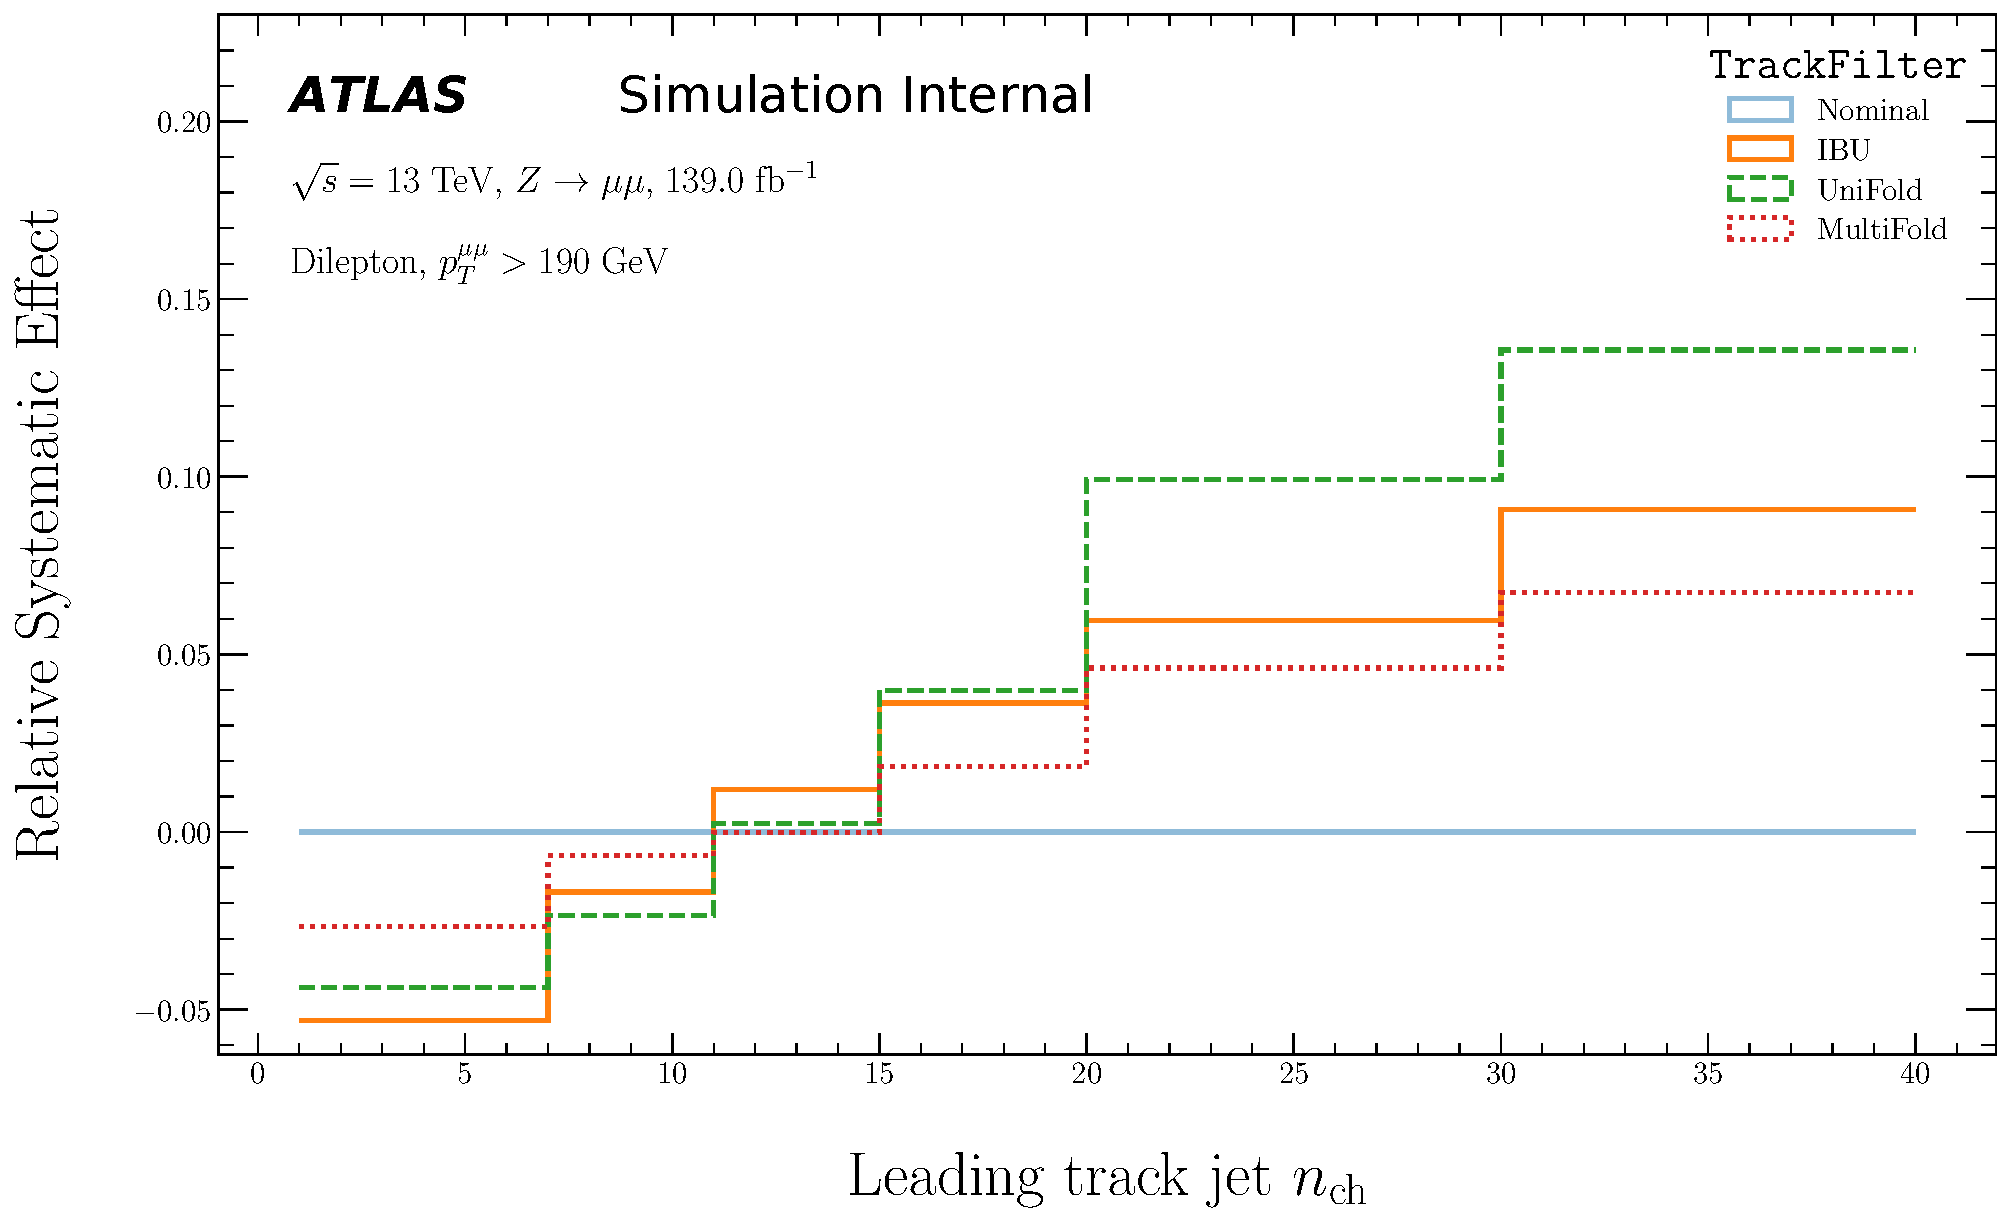
\includegraphics[width=0.25\textwidth,page=1]{figures/SimResults/TrackJet_SystEffect.pdf}\includegraphics[width=0.25\textwidth,page=5]{figures/SimResults/TrackJet_SystEffect.pdf}\includegraphics[width=0.25\textwidth,page=9]{figures/SimResults/TrackJet_SystEffect.pdf}\includegraphics[width=0.25\textwidth,page=13]{figures/SimResults/TrackJet_SystEffect.pdf}\\
\includegraphics[width=0.25\textwidth,page=17]{figures/SimResults/TrackJet_SystEffect.pdf}\includegraphics[width=0.25\textwidth,page=21]{figures/SimResults/TrackJet_SystEffect.pdf}\includegraphics[width=0.25\textwidth,page=25]{figures/SimResults/TrackJet_SystEffect.pdf}\includegraphics[width=0.25\textwidth,page=29]{figures/SimResults/TrackJet_SystEffect.pdf}\\
\includegraphics[width=0.25\textwidth,page=33]{figures/SimResults/TrackJet_SystEffect.pdf}\includegraphics[width=0.25\textwidth,page=37]{figures/SimResults/TrackJet_SystEffect.pdf}\includegraphics[width=0.25\textwidth,page=41]{figures/SimResults/TrackJet_SystEffect.pdf}\includegraphics[width=0.25\textwidth,page=45]{figures/SimResults/TrackJet_SystEffect.pdf}\\
\includegraphics[width=0.25\textwidth,page=49]{figures/SimResults/TrackJet_SystEffect.pdf}\includegraphics[width=0.25\textwidth,page=53]{figures/SimResults/TrackJet_SystEffect.pdf}\includegraphics[width=0.25\textwidth,page=57]{figures/SimResults/TrackJet_SystEffect.pdf}\includegraphics[width=0.25\textwidth,page=61]{figures/SimResults/TrackJet_SystEffect.pdf}\\
\includegraphics[width=0.25\textwidth,page=65]{figures/SimResults/TrackJet_SystEffect.pdf}\includegraphics[width=0.25\textwidth,page=69]{figures/SimResults/TrackJet_SystEffect.pdf}\includegraphics[width=0.25\textwidth,page=73]{figures/SimResults/TrackJet_SystEffect.pdf}\includegraphics[width=0.25\textwidth,page=77]{figures/SimResults/TrackJet_SystEffect.pdf}\\
\includegraphics[width=0.25\textwidth,page=81]{figures/SimResults/TrackJet_SystEffect.pdf}\includegraphics[width=0.25\textwidth,page=85]{figures/SimResults/TrackJet_SystEffect.pdf}\includegraphics[width=0.25\textwidth,page=89]{figures/SimResults/TrackJet_SystEffect.pdf}\includegraphics[width=0.25\textwidth,page=93]{figures/SimResults/TrackJet_SystEffect.pdf}
\caption{The nominal MultiFolded results where Sherpa is used as data and Pythia is used as the simulation. The error bars represent the total uncertainty, which each component added in quadrature.}
\label{fig:simresultsmulti_nominal}
\end{figure}

\begin{figure}[h!]
\centering
\includegraphics[width=0.25\textwidth,page=2]{figures/SimResults/TrackJet_SystEffect.pdf}\includegraphics[width=0.25\textwidth,page=6]{figures/SimResults/TrackJet_SystEffect.pdf}\includegraphics[width=0.25\textwidth,page=10]{figures/SimResults/TrackJet_SystEffect.pdf}\includegraphics[width=0.25\textwidth,page=14]{figures/SimResults/TrackJet_SystEffect.pdf}\\
\includegraphics[width=0.25\textwidth,page=18]{figures/SimResults/TrackJet_SystEffect.pdf}\includegraphics[width=0.25\textwidth,page=22]{figures/SimResults/TrackJet_SystEffect.pdf}\includegraphics[width=0.25\textwidth,page=26]{figures/SimResults/TrackJet_SystEffect.pdf}\includegraphics[width=0.25\textwidth,page=30]{figures/SimResults/TrackJet_SystEffect.pdf}\\
\includegraphics[width=0.25\textwidth,page=34]{figures/SimResults/TrackJet_SystEffect.pdf}\includegraphics[width=0.25\textwidth,page=38]{figures/SimResults/TrackJet_SystEffect.pdf}\includegraphics[width=0.25\textwidth,page=42]{figures/SimResults/TrackJet_SystEffect.pdf}\includegraphics[width=0.25\textwidth,page=46]{figures/SimResults/TrackJet_SystEffect.pdf}\\
\includegraphics[width=0.25\textwidth,page=50]{figures/SimResults/TrackJet_SystEffect.pdf}\includegraphics[width=0.25\textwidth,page=54]{figures/SimResults/TrackJet_SystEffect.pdf}\includegraphics[width=0.25\textwidth,page=58]{figures/SimResults/TrackJet_SystEffect.pdf}\includegraphics[width=0.25\textwidth,page=62]{figures/SimResults/TrackJet_SystEffect.pdf}\\
\includegraphics[width=0.25\textwidth,page=66]{figures/SimResults/TrackJet_SystEffect.pdf}\includegraphics[width=0.25\textwidth,page=70]{figures/SimResults/TrackJet_SystEffect.pdf}\includegraphics[width=0.25\textwidth,page=74]{figures/SimResults/TrackJet_SystEffect.pdf}\includegraphics[width=0.25\textwidth,page=78]{figures/SimResults/TrackJet_SystEffect.pdf}\\
\includegraphics[width=0.25\textwidth,page=82]{figures/SimResults/TrackJet_SystEffect.pdf}\includegraphics[width=0.25\textwidth,page=86]{figures/SimResults/TrackJet_SystEffect.pdf}\includegraphics[width=0.25\textwidth,page=90]{figures/SimResults/TrackJet_SystEffect.pdf}\includegraphics[width=0.25\textwidth,page=94]{figures/SimResults/TrackJet_SystEffect.pdf}
\caption{The nominal MultiFolded results where Sherpa is used as data and Pythia is used as the simulation. The error bars represent the total uncertainty, which each component added in quadrature.}
\label{fig:simresultsmulti_nominal}
\end{figure}

\begin{figure}[h!]
\centering
\includegraphics[width=0.25\textwidth,page=3]{figures/SimResults/TrackJet_SystEffect.pdf}\includegraphics[width=0.25\textwidth,page=7]{figures/SimResults/TrackJet_SystEffect.pdf}\includegraphics[width=0.25\textwidth,page=11]{figures/SimResults/TrackJet_SystEffect.pdf}\includegraphics[width=0.25\textwidth,page=15]{figures/SimResults/TrackJet_SystEffect.pdf}\\
\includegraphics[width=0.25\textwidth,page=19]{figures/SimResults/TrackJet_SystEffect.pdf}\includegraphics[width=0.25\textwidth,page=23]{figures/SimResults/TrackJet_SystEffect.pdf}\includegraphics[width=0.25\textwidth,page=27]{figures/SimResults/TrackJet_SystEffect.pdf}\includegraphics[width=0.25\textwidth,page=31]{figures/SimResults/TrackJet_SystEffect.pdf}\\
\includegraphics[width=0.25\textwidth,page=35]{figures/SimResults/TrackJet_SystEffect.pdf}\includegraphics[width=0.25\textwidth,page=39]{figures/SimResults/TrackJet_SystEffect.pdf}\includegraphics[width=0.25\textwidth,page=43]{figures/SimResults/TrackJet_SystEffect.pdf}\includegraphics[width=0.25\textwidth,page=47]{figures/SimResults/TrackJet_SystEffect.pdf}\\
\includegraphics[width=0.25\textwidth,page=51]{figures/SimResults/TrackJet_SystEffect.pdf}\includegraphics[width=0.25\textwidth,page=55]{figures/SimResults/TrackJet_SystEffect.pdf}\includegraphics[width=0.25\textwidth,page=59]{figures/SimResults/TrackJet_SystEffect.pdf}\includegraphics[width=0.25\textwidth,page=63]{figures/SimResults/TrackJet_SystEffect.pdf}\\
\includegraphics[width=0.25\textwidth,page=67]{figures/SimResults/TrackJet_SystEffect.pdf}\includegraphics[width=0.25\textwidth,page=71]{figures/SimResults/TrackJet_SystEffect.pdf}\includegraphics[width=0.25\textwidth,page=75]{figures/SimResults/TrackJet_SystEffect.pdf}\includegraphics[width=0.25\textwidth,page=79]{figures/SimResults/TrackJet_SystEffect.pdf}\\
\includegraphics[width=0.25\textwidth,page=83]{figures/SimResults/TrackJet_SystEffect.pdf}\includegraphics[width=0.25\textwidth,page=87]{figures/SimResults/TrackJet_SystEffect.pdf}\includegraphics[width=0.25\textwidth,page=91]{figures/SimResults/TrackJet_SystEffect.pdf}\includegraphics[width=0.25\textwidth,page=95]{figures/SimResults/TrackJet_SystEffect.pdf}
\caption{The nominal MultiFolded results where Sherpa is used as data and Pythia is used as the simulation. The error bars represent the total uncertainty, which each component added in quadrature.}
\label{fig:simresultsmulti_nominal}
\end{figure}

\begin{figure}[h!]
\centering
\includegraphics[width=0.25\textwidth,page=4]{figures/SimResults/TrackJet_SystEffect.pdf}\includegraphics[width=0.25\textwidth,page=8]{figures/SimResults/TrackJet_SystEffect.pdf}\includegraphics[width=0.25\textwidth,page=12]{figures/SimResults/TrackJet_SystEffect.pdf}\includegraphics[width=0.25\textwidth,page=16]{figures/SimResults/TrackJet_SystEffect.pdf}\\
\includegraphics[width=0.25\textwidth,page=20]{figures/SimResults/TrackJet_SystEffect.pdf}\includegraphics[width=0.25\textwidth,page=24]{figures/SimResults/TrackJet_SystEffect.pdf}\includegraphics[width=0.25\textwidth,page=28]{figures/SimResults/TrackJet_SystEffect.pdf}\includegraphics[width=0.25\textwidth,page=32]{figures/SimResults/TrackJet_SystEffect.pdf}\\
\includegraphics[width=0.25\textwidth,page=36]{figures/SimResults/TrackJet_SystEffect.pdf}\includegraphics[width=0.25\textwidth,page=40]{figures/SimResults/TrackJet_SystEffect.pdf}\includegraphics[width=0.25\textwidth,page=44]{figures/SimResults/TrackJet_SystEffect.pdf}\includegraphics[width=0.25\textwidth,page=48]{figures/SimResults/TrackJet_SystEffect.pdf}\\
\includegraphics[width=0.25\textwidth,page=52]{figures/SimResults/TrackJet_SystEffect.pdf}\includegraphics[width=0.25\textwidth,page=56]{figures/SimResults/TrackJet_SystEffect.pdf}\includegraphics[width=0.25\textwidth,page=60]{figures/SimResults/TrackJet_SystEffect.pdf}\includegraphics[width=0.25\textwidth,page=64]{figures/SimResults/TrackJet_SystEffect.pdf}\\
\includegraphics[width=0.25\textwidth,page=68]{figures/SimResults/TrackJet_SystEffect.pdf}\includegraphics[width=0.25\textwidth,page=72]{figures/SimResults/TrackJet_SystEffect.pdf}\includegraphics[width=0.25\textwidth,page=76]{figures/SimResults/TrackJet_SystEffect.pdf}\includegraphics[width=0.25\textwidth,page=80]{figures/SimResults/TrackJet_SystEffect.pdf}\\
\includegraphics[width=0.25\textwidth,page=84]{figures/SimResults/TrackJet_SystEffect.pdf}\includegraphics[width=0.25\textwidth,page=88]{figures/SimResults/TrackJet_SystEffect.pdf}\includegraphics[width=0.25\textwidth,page=92]{figures/SimResults/TrackJet_SystEffect.pdf}\includegraphics[width=0.25\textwidth,page=96]{figures/SimResults/TrackJet_SystEffect.pdf}
\caption{The nominal MultiFolded results where Sherpa is used as data and Pythia is used as the simulation. The error bars represent the total uncertainty, which each component added in quadrature.}
\label{fig:simresultsmulti_nominal}
\end{figure}

\begin{comment}
\begin{figure}[h!]
\centering
\includegraphics[width=0.25\textwidth,page=1]{figures/SimResults/MultiFold_TrackJet_SystEffect.pdf}\includegraphics[width=0.25\textwidth,page=2]{figures/SimResults/MultiFold_TrackJet_SystEffect.pdf}\includegraphics[width=0.25\textwidth,page=3]{figures/SimResults/MultiFold_TrackJet_SystEffect.pdf}\includegraphics[width=0.25\textwidth,page=4]{figures/SimResults/MultiFold_TrackJet_SystEffect.pdf}\\
\includegraphics[width=0.25\textwidth,page=5]{figures/SimResults/MultiFold_TrackJet_SystEffect.pdf}\includegraphics[width=0.25\textwidth,page=6]{figures/SimResults/MultiFold_TrackJet_SystEffect.pdf}\includegraphics[width=0.25\textwidth,page=7]{figures/SimResults/MultiFold_TrackJet_SystEffect.pdf}\includegraphics[width=0.25\textwidth,page=8]{figures/SimResults/MultiFold_TrackJet_SystEffect.pdf}\\
\includegraphics[width=0.25\textwidth,page=9]{figures/SimResults/MultiFold_TrackJet_SystEffect.pdf}\includegraphics[width=0.25\textwidth,page=10]{figures/SimResults/MultiFold_TrackJet_SystEffect.pdf}\includegraphics[width=0.25\textwidth,page=11]{figures/SimResults/MultiFold_TrackJet_SystEffect.pdf}\includegraphics[width=0.25\textwidth,page=12]{figures/SimResults/MultiFold_TrackJet_SystEffect.pdf}\\
\includegraphics[width=0.25\textwidth,page=13]{figures/SimResults/MultiFold_TrackJet_SystEffect.pdf}\includegraphics[width=0.25\textwidth,page=14]{figures/SimResults/MultiFold_TrackJet_SystEffect.pdf}\includegraphics[width=0.25\textwidth,page=15]{figures/SimResults/MultiFold_TrackJet_SystEffect.pdf}\includegraphics[width=0.25\textwidth,page=16]{figures/SimResults/MultiFold_TrackJet_SystEffect.pdf}\\
\includegraphics[width=0.25\textwidth,page=17]{figures/SimResults/MultiFold_TrackJet_SystEffect.pdf}\includegraphics[width=0.25\textwidth,page=18]{figures/SimResults/MultiFold_TrackJet_SystEffect.pdf}\includegraphics[width=0.25\textwidth,page=19]{figures/SimResults/MultiFold_TrackJet_SystEffect.pdf}\includegraphics[width=0.25\textwidth,page=20]{figures/SimResults/MultiFold_TrackJet_SystEffect.pdf}\\
\includegraphics[width=0.25\textwidth,page=21]{figures/SimResults/MultiFold_TrackJet_SystEffect.pdf}\includegraphics[width=0.25\textwidth,page=22]{figures/SimResults/MultiFold_TrackJet_SystEffect.pdf}\includegraphics[width=0.25\textwidth,page=23]{figures/SimResults/MultiFold_TrackJet_SystEffect.pdf}\includegraphics[width=0.25\textwidth,page=24]{figures/SimResults/MultiFold_TrackJet_SystEffect.pdf}
\caption{The relative experimental systematic uncertainties from tracking, including the inclusive efficiency uncertainty (\texttt{sys\_TrackFilter}), the dense cores uncertainty (\texttt{sys\_JetTrackFilter}), the fake rate uncertainty (\texttt{sys\_Fake}), and the sagitta bias uncertainty (\texttt{sys\_pTScale}).}
\label{fig:simresultsmulti_trackjetuncertsl}
\end{figure}

\begin{figure}[h!]
\centering
\includegraphics[width=0.25\textwidth,page=1]{figures/SimResults/MultiFold_Lepton_SystEffect.pdf}\includegraphics[width=0.25\textwidth,page=2]{figures/SimResults/MultiFold_Lepton_SystEffect.pdf}\includegraphics[width=0.25\textwidth,page=3]{figures/SimResults/MultiFold_Lepton_SystEffect.pdf}\includegraphics[width=0.25\textwidth,page=4]{figures/SimResults/MultiFold_Lepton_SystEffect.pdf}\\
\includegraphics[width=0.25\textwidth,page=5]{figures/SimResults/MultiFold_Lepton_SystEffect.pdf}\includegraphics[width=0.25\textwidth,page=6]{figures/SimResults/MultiFold_Lepton_SystEffect.pdf}\includegraphics[width=0.25\textwidth,page=7]{figures/SimResults/MultiFold_Lepton_SystEffect.pdf}\includegraphics[width=0.25\textwidth,page=8]{figures/SimResults/MultiFold_Lepton_SystEffect.pdf}\\
\includegraphics[width=0.25\textwidth,page=9]{figures/SimResults/MultiFold_Lepton_SystEffect.pdf}\includegraphics[width=0.25\textwidth,page=10]{figures/SimResults/MultiFold_Lepton_SystEffect.pdf}\includegraphics[width=0.25\textwidth,page=11]{figures/SimResults/MultiFold_Lepton_SystEffect.pdf}\includegraphics[width=0.25\textwidth,page=12]{figures/SimResults/MultiFold_Lepton_SystEffect.pdf}\\
\includegraphics[width=0.25\textwidth,page=13]{figures/SimResults/MultiFold_Lepton_SystEffect.pdf}\includegraphics[width=0.25\textwidth,page=14]{figures/SimResults/MultiFold_Lepton_SystEffect.pdf}\includegraphics[width=0.25\textwidth,page=15]{figures/SimResults/MultiFold_Lepton_SystEffect.pdf}\includegraphics[width=0.25\textwidth,page=16]{figures/SimResults/MultiFold_Lepton_SystEffect.pdf}\\
\includegraphics[width=0.25\textwidth,page=17]{figures/SimResults/MultiFold_Lepton_SystEffect.pdf}\includegraphics[width=0.25\textwidth,page=18]{figures/SimResults/MultiFold_Lepton_SystEffect.pdf}\includegraphics[width=0.25\textwidth,page=19]{figures/SimResults/MultiFold_Lepton_SystEffect.pdf}\includegraphics[width=0.25\textwidth,page=20]{figures/SimResults/MultiFold_Lepton_SystEffect.pdf}\\
\includegraphics[width=0.25\textwidth,page=21]{figures/SimResults/MultiFold_Lepton_SystEffect.pdf}\includegraphics[width=0.25\textwidth,page=22]{figures/SimResults/MultiFold_Lepton_SystEffect.pdf}\includegraphics[width=0.25\textwidth,page=23]{figures/SimResults/MultiFold_Lepton_SystEffect.pdf}\includegraphics[width=0.25\textwidth,page=24]{figures/SimResults/MultiFold_Lepton_SystEffect.pdf}
\caption{The relative experimental systematic uncertainties from the muons.  See Sec.~\ref{sec:muonuncerts} for further details.}
\label{fig:simresultsmulti_muonuncerts}
\end{figure}
\end{comment}

Theory modeling uncertainties are quantified in Figs.~\ref{fig:simresultsmulti_theoryuncertsl} and~\ref{fig:simresultsmulti_theoryQCDuncertsl} for the parton shower and the matrix element, respectively.  For the latter, we have only computed the extreme variations (factorization and renormalization scale both $\times 2$ or $\times 1/2$), which are likely to form the typical envelope over all physically meaningful variations.  Note that we do not have detector-level samples for any of these variations and so these uncertainties are computed by first reweighting the nominal simulation using particle-level-only samples and then (re)running the unfolding procedure.   As expected, the variation of the renormalization scale (which changes the effective $\alpha_s$ in the final state shower) is the most important for many of the observables.

\begin{comment}
\begin{figure}[h!]
\centering
\includegraphics[width=0.25\textwidth,page=1]{figures/SimResults/MultiFold_Theory_SystEffect.pdf}\includegraphics[width=0.25\textwidth,page=2]{figures/SimResults/MultiFold_Theory_SystEffect.pdf}\includegraphics[width=0.25\textwidth,page=3]{figures/SimResults/MultiFold_Theory_SystEffect.pdf}\includegraphics[width=0.25\textwidth,page=4]{figures/SimResults/MultiFold_Theory_SystEffect.pdf}\\
\includegraphics[width=0.25\textwidth,page=5]{figures/SimResults/MultiFold_Theory_SystEffect.pdf}\includegraphics[width=0.25\textwidth,page=6]{figures/SimResults/MultiFold_Theory_SystEffect.pdf}\includegraphics[width=0.25\textwidth,page=7]{figures/SimResults/MultiFold_Theory_SystEffect.pdf}\includegraphics[width=0.25\textwidth,page=8]{figures/SimResults/MultiFold_Theory_SystEffect.pdf}\\
\includegraphics[width=0.25\textwidth,page=9]{figures/SimResults/MultiFold_Theory_SystEffect.pdf}\includegraphics[width=0.25\textwidth,page=10]{figures/SimResults/MultiFold_Theory_SystEffect.pdf}\includegraphics[width=0.25\textwidth,page=11]{figures/SimResults/MultiFold_Theory_SystEffect.pdf}\includegraphics[width=0.25\textwidth,page=12]{figures/SimResults/MultiFold_Theory_SystEffect.pdf}\\
\includegraphics[width=0.25\textwidth,page=13]{figures/SimResults/MultiFold_Theory_SystEffect.pdf}\includegraphics[width=0.25\textwidth,page=14]{figures/SimResults/MultiFold_Theory_SystEffect.pdf}\includegraphics[width=0.25\textwidth,page=15]{figures/SimResults/MultiFold_Theory_SystEffect.pdf}\includegraphics[width=0.25\textwidth,page=16]{figures/SimResults/MultiFold_Theory_SystEffect.pdf}\\
\includegraphics[width=0.25\textwidth,page=17]{figures/SimResults/MultiFold_Theory_SystEffect.pdf}\includegraphics[width=0.25\textwidth,page=18]{figures/SimResults/MultiFold_Theory_SystEffect.pdf}\includegraphics[width=0.25\textwidth,page=19]{figures/SimResults/MultiFold_Theory_SystEffect.pdf}\includegraphics[width=0.25\textwidth,page=20]{figures/SimResults/MultiFold_Theory_SystEffect.pdf}\\
\includegraphics[width=0.25\textwidth,page=21]{figures/SimResults/MultiFold_Theory_SystEffect.pdf}\includegraphics[width=0.25\textwidth,page=22]{figures/SimResults/MultiFold_Theory_SystEffect.pdf}\includegraphics[width=0.25\textwidth,page=23]{figures/SimResults/MultiFold_Theory_SystEffect.pdf}\includegraphics[width=0.25\textwidth,page=24]{figures/SimResults/MultiFold_Theory_SystEffect.pdf}
\caption{The relative theory systematic uncertainties related to the parton shower.}
\label{fig:simresultsmulti_theoryuncertsl}
\end{figure}

\begin{figure}[h!]
\centering
\includegraphics[width=0.25\textwidth,page=1]{figures/SimResults/MultiFold_QCD_SystEffect.pdf}\includegraphics[width=0.25\textwidth,page=2]{figures/SimResults/MultiFold_QCD_SystEffect.pdf}\includegraphics[width=0.25\textwidth,page=3]{figures/SimResults/MultiFold_QCD_SystEffect.pdf}\includegraphics[width=0.25\textwidth,page=4]{figures/SimResults/MultiFold_QCD_SystEffect.pdf}\\
\includegraphics[width=0.25\textwidth,page=5]{figures/SimResults/MultiFold_QCD_SystEffect.pdf}\includegraphics[width=0.25\textwidth,page=6]{figures/SimResults/MultiFold_QCD_SystEffect.pdf}\includegraphics[width=0.25\textwidth,page=7]{figures/SimResults/MultiFold_QCD_SystEffect.pdf}\includegraphics[width=0.25\textwidth,page=8]{figures/SimResults/MultiFold_QCD_SystEffect.pdf}\\
\includegraphics[width=0.25\textwidth,page=9]{figures/SimResults/MultiFold_QCD_SystEffect.pdf}\includegraphics[width=0.25\textwidth,page=10]{figures/SimResults/MultiFold_QCD_SystEffect.pdf}\includegraphics[width=0.25\textwidth,page=11]{figures/SimResults/MultiFold_QCD_SystEffect.pdf}\includegraphics[width=0.25\textwidth,page=12]{figures/SimResults/MultiFold_QCD_SystEffect.pdf}\\
\includegraphics[width=0.25\textwidth,page=13]{figures/SimResults/MultiFold_QCD_SystEffect.pdf}\includegraphics[width=0.25\textwidth,page=14]{figures/SimResults/MultiFold_QCD_SystEffect.pdf}\includegraphics[width=0.25\textwidth,page=15]{figures/SimResults/MultiFold_QCD_SystEffect.pdf}\includegraphics[width=0.25\textwidth,page=16]{figures/SimResults/MultiFold_QCD_SystEffect.pdf}\\
\includegraphics[width=0.25\textwidth,page=17]{figures/SimResults/MultiFold_QCD_SystEffect.pdf}\includegraphics[width=0.25\textwidth,page=18]{figures/SimResults/MultiFold_QCD_SystEffect.pdf}\includegraphics[width=0.25\textwidth,page=19]{figures/SimResults/MultiFold_QCD_SystEffect.pdf}\includegraphics[width=0.25\textwidth,page=20]{figures/SimResults/MultiFold_QCD_SystEffect.pdf}\\
\includegraphics[width=0.25\textwidth,page=21]{figures/SimResults/MultiFold_QCD_SystEffect.pdf}\includegraphics[width=0.25\textwidth,page=22]{figures/SimResults/MultiFold_QCD_SystEffect.pdf}\includegraphics[width=0.25\textwidth,page=23]{figures/SimResults/MultiFold_QCD_SystEffect.pdf}\includegraphics[width=0.25\textwidth,page=24]{figures/SimResults/MultiFold_QCD_SystEffect.pdf}
\caption{The relative theory systematic uncertainties in the matrix elements.}
\label{fig:simresultsmulti_theoryQCDuncertsl}
\end{figure}
\end{comment}
